\documentclass{standalone}
\usepackage{tikz}
\usetikzlibrary{patterns, positioning}
\usepackage[sfdefault]{ClearSans} %% option 'sfdefault' activates Clear Sans as the default text font
\usepackage[T1]{fontenc}

\begin{document}
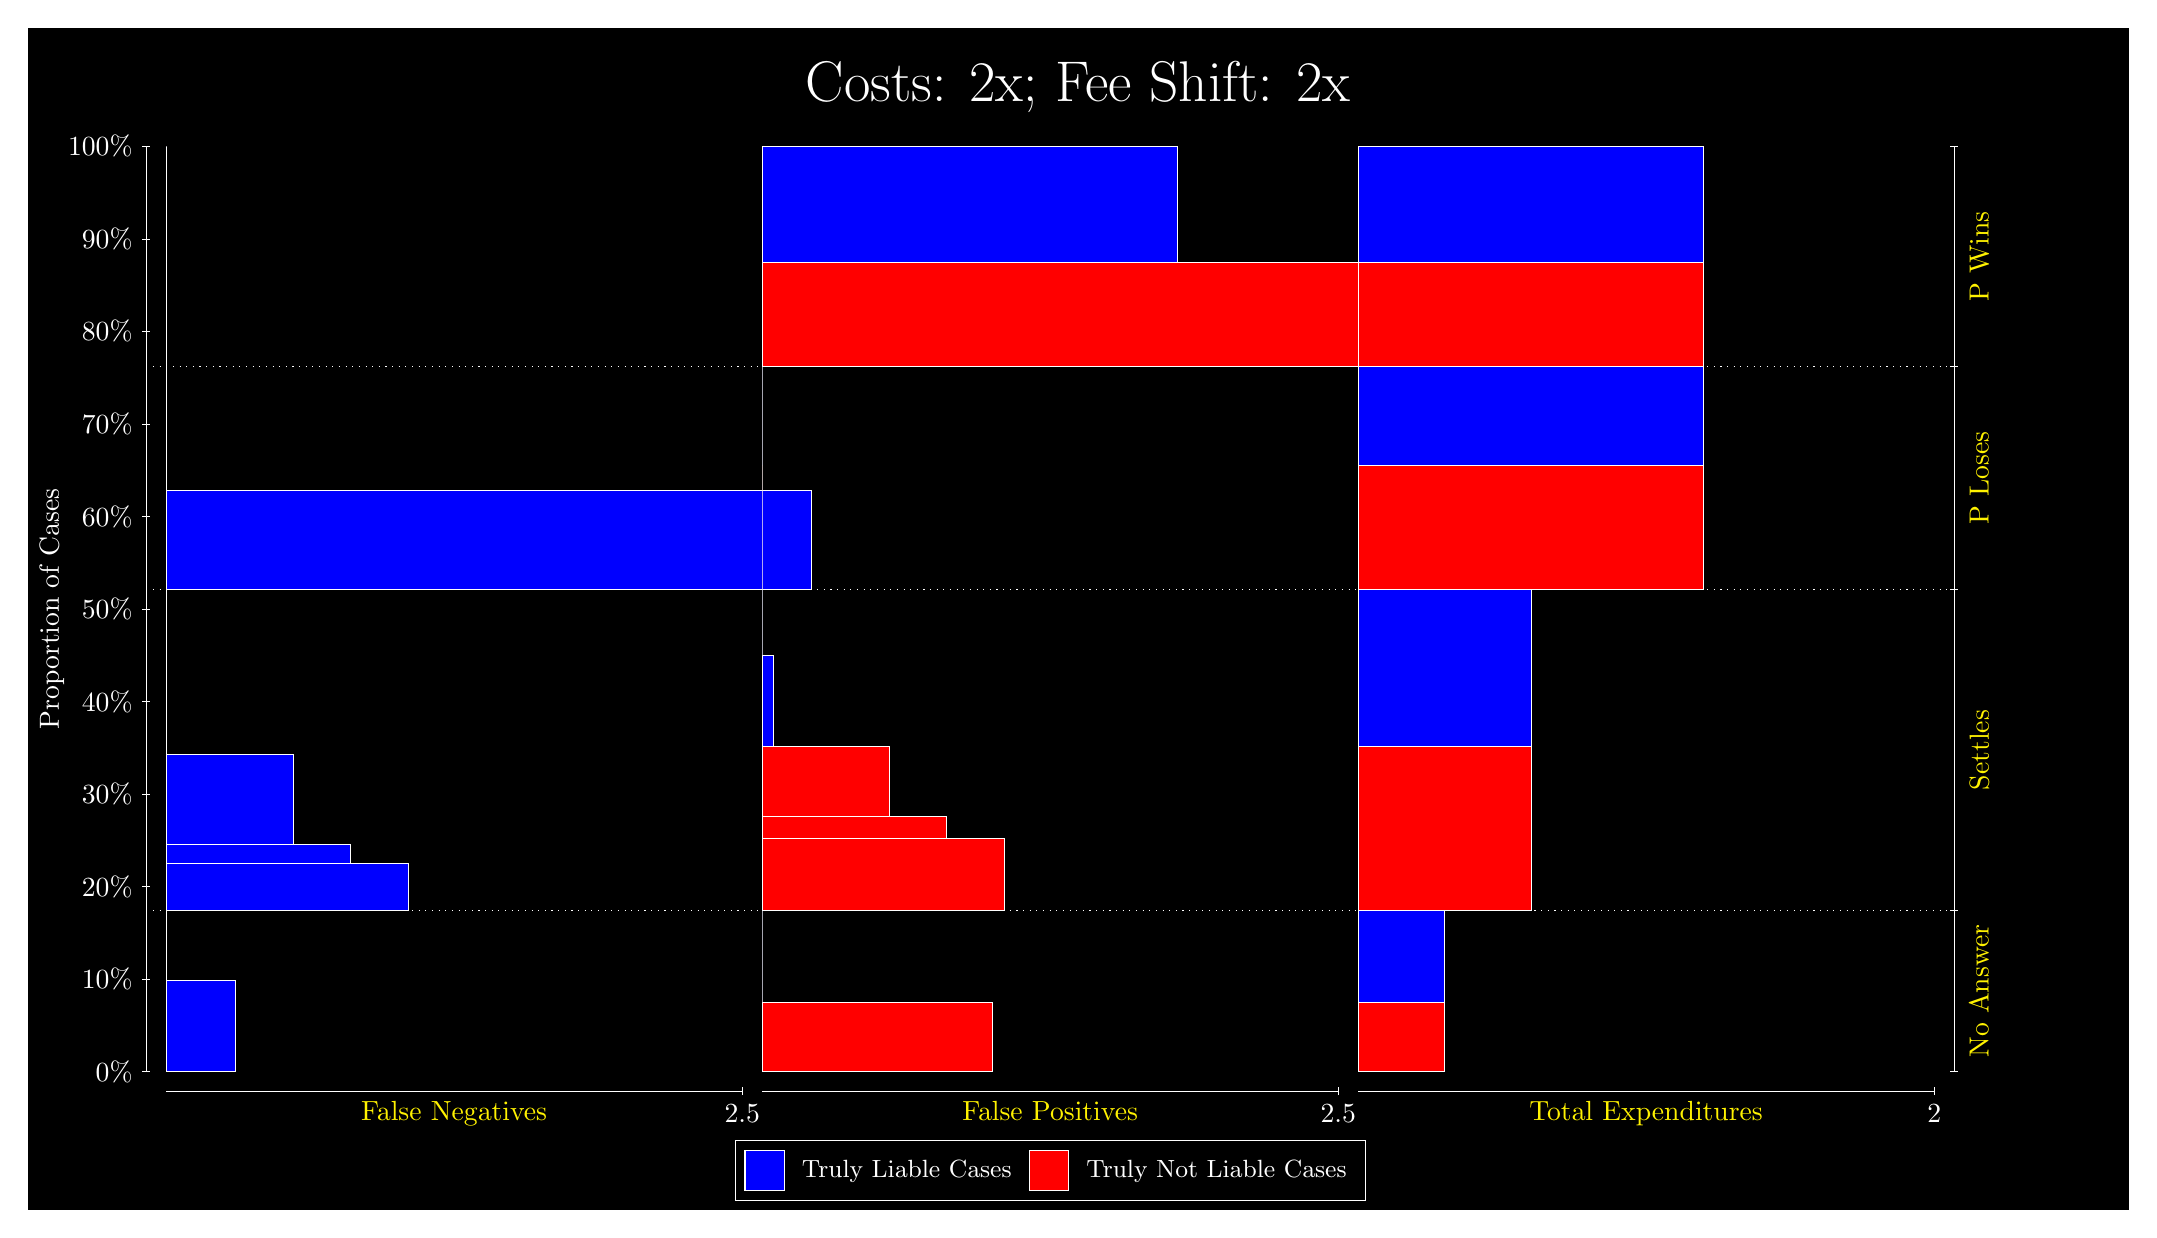
\begin{tikzpicture}
\draw[fill=black] (0,0) rectangle (26.667,15);
\draw[text=white] (0,13.5) rectangle (26.667,15) node[midway] {\huge Costs: 2x; Fee Shift: 2x};
\draw[white, very thin] (1.5,1.75) -- (1.5,13.5);
\node[rotate=90, text=white, anchor=center] at (0.3, 7.625) {Proportion of Cases};
\draw[white, very thin] (1.45,1.75) -- (1.55,1.75);
\node[text=white, anchor=east] at (1.45, 1.75) {0\%};
\draw[white, very thin] (1.45,2.925) -- (1.55,2.925);
\node[text=white, anchor=east] at (1.45, 2.925) {10\%};
\draw[white, very thin] (1.45,4.1) -- (1.55,4.1);
\node[text=white, anchor=east] at (1.45, 4.1) {20\%};
\draw[white, very thin] (1.45,5.275) -- (1.55,5.275);
\node[text=white, anchor=east] at (1.45, 5.275) {30\%};
\draw[white, very thin] (1.45,6.45) -- (1.55,6.45);
\node[text=white, anchor=east] at (1.45, 6.45) {40\%};
\draw[white, very thin] (1.45,7.625) -- (1.55,7.625);
\node[text=white, anchor=east] at (1.45, 7.625) {50\%};
\draw[white, very thin] (1.45,8.8) -- (1.55,8.8);
\node[text=white, anchor=east] at (1.45, 8.8) {60\%};
\draw[white, very thin] (1.45,9.975) -- (1.55,9.975);
\node[text=white, anchor=east] at (1.45, 9.975) {70\%};
\draw[white, very thin] (1.45,11.15) -- (1.55,11.15);
\node[text=white, anchor=east] at (1.45, 11.15) {80\%};
\draw[white, very thin] (1.45,12.325) -- (1.55,12.325);
\node[text=white, anchor=east] at (1.45, 12.325) {90\%};
\draw[white, very thin] (1.45,13.5) -- (1.55,13.5);
\node[text=white, anchor=east] at (1.45, 13.5) {100\%};

\draw[white, very thin] (24.457,1.75) -- (24.457,13.5);
\draw[white, very thin] (24.407,1.75) -- (24.507,1.75);
\node[anchor=west] at (24.407, 1.75) {};
\draw[white, very thin] (24.407,3.7924) -- (24.507,3.7924);
\node[anchor=west] at (24.407, 3.7924) {};
\draw[white, very thin] (24.407,7.8756) -- (24.507,7.8756);
\node[anchor=west] at (24.407, 7.8756) {};
\draw[white, very thin] (24.407,10.701) -- (24.507,10.701);
\node[anchor=west] at (24.407, 10.701) {};
\draw[white, very thin] (24.407,13.5) -- (24.507,13.5);
\node[anchor=west] at (24.407, 13.5) {};

\draw[white, very thin, fill=blue] (1.75,1.75) rectangle (2.6283,2.9121);
\draw[white, very thin, fill=red] (1.75,2.9121) rectangle (1.75,3.7924);
\draw[white, very thin, fill=blue] (1.75,3.7924) rectangle (4.8239,4.3914);
\draw[white, very thin, fill=blue] (1.75,4.3914) rectangle (4.092,4.638);
\draw[white, very thin, fill=blue] (1.75,4.638) rectangle (3.3602,5.7823);
\draw[white, very thin, fill=red] (1.75,5.7823) rectangle (1.75,7.8756);
\draw[white, very thin, fill=blue] (1.75,7.8756) rectangle (9.9471,9.127);
\draw[white, very thin, fill=red] (1.75,9.127) rectangle (1.75,10.701);
\draw[white, very thin, fill=red] (1.75,10.701) rectangle (1.75,12.028);
\draw[white, very thin, fill=blue] (1.75,12.028) rectangle (1.75,13.5);
\draw[white, very thin, fill=red] (9.3189,1.75) rectangle (12.246,2.6303);
\draw[white, very thin, fill=blue] (9.3189,2.6303) rectangle (9.3189,3.7924);
\draw[white, very thin, fill=red] (9.3189,3.7924) rectangle (12.393,4.7173);
\draw[white, very thin, fill=red] (9.3189,4.7173) rectangle (11.661,4.9958);
\draw[white, very thin, fill=red] (9.3189,4.9958) rectangle (10.929,5.8858);
\draw[white, very thin, fill=blue] (9.3189,5.8858) rectangle (9.4652,7.0301);
\draw[white, very thin, fill=blue] (9.3189,7.0301) rectangle (9.3189,7.8756);
\draw[white, very thin, fill=red] (9.3189,7.8756) rectangle (9.3189,9.4501);
\draw[white, very thin, fill=blue] (9.3189,9.4501) rectangle (9.3189,10.701);
\draw[white, very thin, fill=red] (9.3189,10.701) rectangle (17.516,12.028);
\draw[white, very thin, fill=blue] (9.3189,12.028) rectangle (14.588,13.5);
\draw[white, very thin, fill=red] (16.888,1.75) rectangle (17.986,2.6303);
\draw[white, very thin, fill=blue] (16.888,2.6303) rectangle (17.986,3.7924);
\draw[white, very thin, fill=red] (16.888,3.7924) rectangle (19.083,5.8858);
\draw[white, very thin, fill=blue] (16.888,5.8858) rectangle (19.083,7.8756);
\draw[white, very thin, fill=red] (16.888,7.8756) rectangle (21.279,9.4501);
\draw[white, very thin, fill=blue] (16.888,9.4501) rectangle (21.279,10.701);
\draw[white, very thin, fill=red] (16.888,10.701) rectangle (21.279,12.028);
\draw[white, very thin, fill=blue] (16.888,12.028) rectangle (21.279,13.5);
\draw[white, dotted] (1.5,3.7924) -- (24.457,3.7924);
\draw[white, dotted] (1.5,7.8756) -- (24.457,7.8756);
\draw[white, dotted] (1.5,10.701) -- (24.457,10.701);
\draw[white, very thin] (1.75,1.5) -- (9.0689,1.5);
\node[text=yellow, anchor=north] at (5.4094, 1.5) {False Negatives};
\draw[white, very thin] (9.0689,1.45) -- (9.0689,1.55);
\node[text=white, anchor=north] at (9.0689, 1.45) {2.5};

\draw[white, very thin] (9.3189,1.5) -- (16.638,1.5);
\node[text=yellow, anchor=north] at (12.978, 1.5) {False Positives};
\draw[white, very thin] (16.638,1.45) -- (16.638,1.55);
\node[text=white, anchor=north] at (16.638, 1.45) {2.5};

\draw[white, very thin] (16.888,1.5) -- (24.207,1.5);
\node[text=yellow, anchor=north] at (20.547, 1.5) {Total Expenditures};
\draw[white, very thin] (24.207,1.45) -- (24.207,1.55);
\node[text=white, anchor=north] at (24.207, 1.45) {2};

\node[text=yellow, centered, rotate=90] at (24.777, 2.7712) {No Answer};
\node[text=yellow, centered, rotate=90] at (24.777, 5.834) {Settles};
\node[text=yellow, centered, rotate=90] at (24.777, 9.2886) {P Loses};
\node[text=yellow, centered, rotate=90] at (24.777, 12.101) {P Wins};

\draw (12.978300999999998,1.5) node[draw=none] (baseCoordinate) {};
\begin{scope}[align=center]
        \matrix[scale=0.5, draw=white, below=0.5cm of baseCoordinate, nodes={draw}, column sep=0.1cm]{
            \node[rectangle, draw, minimum width=0.5cm, minimum height=0.5cm, fill=blue] {}; &
            \node[draw=none, font=\small, text=white] (B) {Truly Liable Cases}; &
            \node[rectangle, draw, minimum width=0.5cm, minimum height=0.5cm, fill=red] {}; &
            \node[draw=none, font=\small, text=white] (B) {Truly Not Liable Cases}; \\
            };
\end{scope}

\end{tikzpicture}
\end{document}